\documentclass[lettersize,journal]{IEEEtran}

\usepackage{amsmath,amssymb,amsfonts}
\usepackage{graphicx}
\usepackage{booktabs}
\usepackage{array}
\usepackage{tikz}
\usetikzlibrary{shapes,arrows.meta,positioning,calc}
\usepackage{siunitx}
\usepackage{multirow}
\usepackage{cite}
\usepackage{float}
\usepackage{url}
\def\UrlBreaks{\do\/\do\.\do\-\do\_\do\?\do\=\do\&}

% ------------------------------------------------------------------
% Helper macros
% ------------------------------------------------------------------
\newcommand{\kohm}{\,\text{k}\Omega}
\newcommand{\code}[1]{\texttt{\detokenize{#1}}}
\newcommand{\Ts}{T_{\!s}}
\newcommand{\Kcr}{K_{\mathrm{cr}}}
\newcommand{\wcr}{\omega_{\mathrm{cr}}}
\newcommand{\Pcr}{P_{\mathrm{cr}}}
\newcommand{\rpm}{\,\text{rpm}}
% Figure box: shows the image if the file exists, otherwise a labelled placeholder.
% usage: \figbox{file}{width}{placeholder height}
\newcommand{\figbox}[3]{%
  \IfFileExists{#1}{\includegraphics[width=#2]{#1}}{%
    \fbox{\parbox[c][#3][c]{\dimexpr#2-2\fboxsep-2\fboxrule\relax}{\centering\footnotesize\textsf{[Insert image]}\\[2pt]\texttt{\detokenize{#1}}}}}}

\begin{document}

% =============================== COVER PAGE ===============================
\begin{titlepage}
\thispagestyle{empty}

\begin{center}
{\Large\bfseries STEADY-STATE ERROR USING ROOT LOCUS DESIGN}\\[10pt]
{\large Experiment No. 9}
\end{center}

\vspace{1.2cm}
\noindent
\begin{tabular}{@{}p{3.6cm}l@{}}
Course Code & : EE302 \\[3pt]
Course Name & : Control Systems Laboratory \\[3pt]
Department & : School of Computing and Electrical Engineering \\[3pt]
Institute & : Indian Institute of Technology Mandi \\[3pt]
Course Instructor & : Dr. Yanumula Venkata Karteek \\[3pt]
Teaching Assistant & : \\[3pt]
Date of Experiment & : 28\textsuperscript{th} October, 2026 \hspace{3.2cm} Submission Date : 3\textsuperscript{rd} November, 2026 \\[3pt]
Group Number & : 22 \\
\end{tabular}

\vspace{1.5cm}
\begin{center}
{\bfseries GROUP MEMBER DETAILS}\\[8pt]
\begin{tabular}{@{}clll@{}}
\toprule
S.No. & Name & Roll No. & Signature \\
\midrule
1 & Neil Bakshi & B24344 & \\[6pt]
2 & Ritvik Garg & B24349 & \\[6pt]
3 & Saurabh Gopal & B24352 & \\[6pt]
4 & Snehal Narendra Patil & B24353 & \\[6pt]
\bottomrule
\end{tabular}
\end{center}

\vfill
\begin{center}
August--December 2026
\end{center}

\end{titlepage}

\title{Steady-State Error Using Root Locus Design}

\author{Neil~Bakshi,
        Ritvik~Garg,
        Saurabh~Gopal,
        and~Snehal~Narendra~Patil
        \IEEEcompsocitemizethanks{
        \IEEEcompsocthanksitem All authors are with the School of Computing and Electrical Engineering, Indian Institute of Technology Mandi, Himachal Pradesh, India.}}

\markboth{EE302: Control Systems Laboratory, Group 22, August--December 2026}{}

\maketitle

% ================================ ABSTRACT ================================
\begin{abstract}
This report documents the design of proportional (P), proportional--integral (PI) and proportional--integral--derivative (PID) speed controllers for a DC encoder motor using root locus and Ziegler--Nichols tuning. The motor was driven by an L298N from a $12\,\text{V}$ supply and controlled by an Arduino Mega 2560 at a sample time of $0.02\,\text{s}$. A third-order model, $G(s)=7.3108\times10^{6}/(s^3+55.2546s^2+3570.6s+6.877\times10^{4})$ in rpm per normalised volt, was fitted to a $2.5\,\text{s}$ window of one $5\,\text{V}$ open-loop step (measured; fit $64.38\%$; model DC gain $106.3$ against $108.9\rpm/\text{V}$ measured). On this model the Routh test and \code{allmargin} give $\Kcr=0.0176$, $\wcr=59.75\,\text{rad/s}$ and $\Pcr=0.1051\,\text{s}$, and the sampled loop has $\Kcr=0.0132$ (simulated). No proportional gain gives $\zeta=0.707$ or $\zeta=0.456$, no critical damping exists, and every stable P gain leaves a step error of at least $34.9\%$ (derived). The Ziegler--Nichols gains are $K_p=0.00879$ (P); $K_p=0.00791$, $T_i=0.0876\,\text{s}$ (PI); and $K_p=0.01055$, $T_i=0.0526\,\text{s}$, $T_d=0.0131\,\text{s}$ (PID); all three loops are stable in simulation. On hardware, with a $270\rpm$ reference and one run per controller, the final speeds were $184.65$, $270.17$ and $270.67\rpm$, i.e.\ errors of $31.61\%$, $-0.06\%$ and $-0.25\%$ (measured), against $51.69\%$, $0$ and $0$ in simulation. The PID response peaked at $368.8\rpm$, $36.6\%$ above the reference, close to the sampled simulation ($355.7\rpm$). The P error is smaller than simulated because the static gain at the hardware operating points is about $2.3$ to $2.5$ times the identified gain (derived from the logs). A persistent speed ripple of $56.3$, $75.0$ and $112.5\rpm$ peak to peak, absent from the noise-free simulation, was observed; its cause was not isolated. The Task~1b hardware check and any detuning of the Ziegler--Nichols gains were not performed.
\end{abstract}

\begin{IEEEkeywords}
Steady-state error, root locus, Ziegler--Nichols tuning, PID controller, system identification, critical gain, encoder quantization, DC motor, L298N, Arduino Mega 2560.
\end{IEEEkeywords}

% ============================== INTRODUCTION ==============================
\section{Introduction}
A feedback controller makes the output follow a reference with a small steady-state error while keeping the loop stable. For a type-0 plant, proportional control leaves a finite step error that falls as the gain rises, but a larger gain moves the closed-loop poles toward the imaginary axis; an integral term removes the error at the cost of an extra pole and phase lag~\cite{ogata,franklin}. The root locus shows how the closed-loop poles move with the gain and gives the critical gain and frequency at which the loop oscillates at constant amplitude. The Ziegler--Nichols ultimate-gain rules turn these two numbers into P, PI and PID settings~\cite{zn,ogata}.

This experiment applies these ideas to the speed of a DC encoder motor~\cite{labmanual}. Task~1a identifies a third-order transfer function from a measured open-loop step. Task~1b repeats Pre-Lab Question~2 on that model: the stable gain range, the gains for given damping ratios, critical damping and sustained oscillation. Task~2a reads $\Kcr$, $\wcr$ and $\Pcr$ from the root locus and from the Routh test. Task~2b builds the Ziegler--Nichols P, PI and PID controllers and compares their simulated responses, first on the linear continuous model and then on a sampled model with actuator limits. Task~2c runs the three controllers on the motor. The manual itself has two headed tasks: Task~1 (proportional design, Tasks~1a and 1b here) and Task~2 (PID design, Tasks~2a to 2c here).

The hardware part was limited. The driver was an L298N without a series resistor; the open-loop step had to be shortened to $5\,\text{s}$ because the speed fell in longer runs; each controller was run once, at one reference ($270\rpm$); the Task~1b hardware check was not run; and the Ziegler--Nichols gains were not detuned. Every number in this report is tagged as measured, simulated, derived or not obtained (Section~\ref{sec:status}), and benchmark values from the manual's reference identification are shown only as labelled benchmark references.

% =========================== LEARNING OBJECTIVES ===========================
\section{Learning Objectives}
\begin{itemize}
\item To identify a third-order transfer function of a DC motor from a measured step response and judge the quality of the fit.
\item To use the root locus and the Routh test to find the stable gain range, the critical gain and frequency, and the damping a proportional loop can reach, and to relate the gain to the steady-state error of a type-0 plant.
\item To design P, PI and PID controllers with the Ziegler--Nichols rules and compare rise time, overshoot and steady-state error in simulation.
\item To run the three controllers on the motor and compare the measured response with the linear and the sampled, saturated simulations.
\item To identify the sources of difference between simulation and hardware: sampling delay, quantization, noise, operating-point gain and driver limits.
\end{itemize}

% ================================= THEORY =================================
\section{Theory}

\subsection{Steady-State Error and System Type}
\label{sec:ess}
For a unity-feedback loop with loop transfer function $L(s)$, the error is $E(s)=R(s)/(1+L(s))$. For a stable closed loop the final-value theorem gives $e_{ss}=\lim_{s\to0}sE(s)$, and for a unit step
\begin{equation}
e_{ss}=\frac{1}{1+K_{pos}},\qquad K_{pos}=L(0).
\label{eq:ess}
\end{equation}
The manual uses $K_p$ both for this position error constant and for the proportional gain; here $K_{pos}$ is the error constant and $K_p$ is the PID proportional gain.

The identified motor model has the form $G(s)=b_0/(s^3+a_2s^2+a_1s+a_0)$ with no pole at the origin, so it is type~0 and $G(0)=b_0/a_0$ is finite. With a proportional gain $K$, $K_{pos}=KG(0)$ and
\begin{equation}
e_{ss}=\frac{1}{1+KG(0)}>0\quad\text{for every finite }K.
\label{eq:essP}
\end{equation}
If the controller contains an integrator, $C(s)=K_p\bigl(1+1/(T_is)+\cdots\bigr)$ has a pole at $s=0$, $L(s)\to\infty$ as $s\to0$, the loop is type~1 and $e_{ss}=0$ for a step, provided the loop is stable. The integrator also adds a pole and phase lag, so its time constant has to be chosen with the rest of the loop~\cite{ogata,franklin}.

\subsection{Root Locus, Routh Test and the Critical Gain}
The closed-loop poles of $1+KG(s)=0$ are the roots of $D(s)+KN(s)=0$ for $G=N/D$. For $G(s)=b_0/(s^3+a_2s^2+a_1s+a_0)$ the characteristic equation is
\begin{equation}
s^3+a_2s^2+a_1s+(a_0+Kb_0)=0,
\label{eq:char}
\end{equation}
with the Routh array
\[
\small
\begin{array}{c|cc}
s^3 & 1 & a_1\\
s^2 & a_2 & a_0+Kb_0\\
s^1 & \dfrac{a_2a_1-a_0-Kb_0}{a_2} & 0\\
s^0 & a_0+Kb_0 &
\end{array}
\]
All first-column entries are positive for $0<K<\Kcr$, where
\begin{equation}
\Kcr=\frac{a_2a_1-a_0}{b_0},\qquad
\wcr=\sqrt{a_1},\qquad
\Pcr=\frac{2\pi}{\wcr}.
\label{eq:kcr}
\end{equation}
At $K=\Kcr$ the $s^1$ entry vanishes, the auxiliary polynomial $a_2s^2+a_0+\Kcr b_0=a_2s^2+a_2a_1$ gives $s=\pm j\sqrt{a_1}$, and the output oscillates at constant amplitude with period $\Pcr$ (the manual's Eq.~(1)). The third closed-loop pole is then at $-a_2$, because the three poles sum to $-a_2$.

The number of poles matters. With $n-m=2$ the asymptotes are at $\pm90^\circ$ with a negative centroid, so the locus never reaches the imaginary axis and $\Kcr$ does not exist. With $n-m=3$ the asymptotes are at $\pm60^\circ$ and $180^\circ$, the two at $\pm60^\circ$ lean into the right half-plane, and the locus must cross the imaginary axis. This is why the manual asks for three poles.

Design targets for a dominant pair $-\sigma\pm j\omega_d$ are read from the second-order relations
\begin{equation}
\mathrm{OS}=e^{-\pi\zeta/\sqrt{1-\zeta^2}},\qquad
\zeta=\frac{-\ln\mathrm{OS}}{\sqrt{\pi^2+\ln^2\mathrm{OS}}},
\label{eq:os}
\end{equation}
which give $\zeta=0.456$ for $20\%$ overshoot; the other target is $\zeta=0.707$. They are approximations that hold when the remaining pole is far from the dominant pair~\cite{ogata}. Critical damping needs a breakaway point on the real axis with $0<K<\Kcr$, i.e.\ a real root of $dK/ds=0$ with $K(s)=-D(s)/b_0$, which for the third-order model reduces to
\begin{equation}
3s^2+2a_2s+a_1=0.
\label{eq:breakaway}
\end{equation}

\subsection{Ziegler--Nichols Tuning and PID Forms}
The ultimate-gain method raises a proportional gain until the loop oscillates steadily, records $\Kcr$ and $\Pcr$, and sets the controller from Table~\ref{tab:zn_rules}~\cite{zn,ogata}. The rules are empirical and aim at a response whose amplitude decays by about a quarter per cycle, which usually means considerable overshoot rather than a minimum-overshoot design.
\begin{table}[H]
\centering
\caption{Ziegler--Nichols ultimate-gain rules (as in the manual's Table~1).}
\label{tab:zn_rules}
\begin{tabular}{@{}cccc@{}}
\toprule
Controller & $K_p$ & $T_i$ & $T_d$ \\
\midrule
P   & $0.5\Kcr$  & $\infty$ & $0$ \\
PI  & $0.45\Kcr$ & $\Pcr/1.2$ & $0$ \\
PID & $0.6\Kcr$  & $0.5\Pcr$ & $0.125\Pcr$ \\
\bottomrule
\end{tabular}
\end{table}
The PID controller is written in the ideal and the parallel forms,
\begin{equation}
C(s)=K_p\Bigl(1+\frac{1}{T_is}+T_ds\Bigr)=K_p+\frac{K_i}{s}+K_ds,
\label{eq:pid}
\end{equation}
with $K_i=K_p/T_i$ and $K_d=K_pT_d$; the manual's $K_1,K_2,K_3$ correspond to $K_p,K_i,K_d$. In the implemented controller the derivative is filtered, $K_dNs/(s+N)$, with $N$ the filter pole in rad/s. The PI controller has a pole at the origin and a zero at $-1/T_i=-1.2/\Pcr$. With $T_i=4T_d$ the PID numerator is $T_iT_ds^2+T_is+1=(2T_ds+1)^2$, a double zero at $-1/(2T_d)=-4/\Pcr$. These are the pole and zero locations of $L(s)=C(s)G(s)$ on the root locus of the PI and PID loops. In the continuous linear model $K_p=0.5\Kcr$ is a gain margin of $2$.

\subsection{The Motor and the Third-Order Model}
A permanent-magnet DC motor obeys $v=Ri+L\,di/dt+K_e\omega$ and $J\,d\omega/dt=K_ti-b\omega$, which gives the second-order transfer function $\Omega(s)/V(s)=K_t/[(Ls+R)(Js+b)+K_tK_e]$. When $L$ is small this behaves like a first-order lag. In the experiment the measured signal also passes through the speed estimator (pulse counting over one sample), the filter $1/(0.02s+1)$ and the PWM and driver stage. The third pole of the identified model absorbs these extra dynamics, and it is also what makes the Ziegler--Nichols method applicable. A complex pair in the identified model is allowed by the fit and has to be judged by how well the model reproduces the measured step, not by a physical interpretation.

\subsection{Sampling, Quantization, Saturation and Windup}
\emph{Sampling delay.} A zero-order hold of period $\Ts$ delays the command by about $\Ts/2$ and adds a phase lag $\omega\Ts/2$. At $\wcr\approx59.75\,\text{rad/s}$ and $\Ts=0.02\,\text{s}$ this is $0.598\,\text{rad}=34.2^\circ$, so the critical gain of the sampled loop is lower than the continuous one. It is found as the gain at which the largest eigenvalue of the discretised closed loop reaches magnitude one.

\emph{Quantization.} The speed is computed from the number of encoder edges $\Delta N$ in one sample,
\begin{equation}
\omega_{\mathrm{rpm}}=\frac{60\,\Delta N}{480\,\Ts},\quad
\Delta\omega_{\mathrm{rpm}}=\frac{60}{480\cdot0.02}=6.25\rpm,
\label{eq:quant}
\end{equation}
where $\Delta\omega_{\mathrm{rpm}}$ is the speed step of one count and $480$ pulses per revolution on one channel is the value used in the lab model. A derivative term differentiates these steps, so the derivative has to be filtered.

\emph{Saturation and windup.} The controller output is limited to $[0,5]$ normalised volts: the drive is unipolar, so a negative command is clipped at zero and the motor cannot be braked actively. While the output is saturated the integrator would keep accumulating error; clamping anti-windup stops the integration while the output is saturated and the error pushes further into the limit. Within the unsaturated band the linear root-locus predictions apply.

% ============================ EXPERIMENTAL SETUP ============================
\section{Experimental Setup}

\subsection{Apparatus and Software}
\begin{table}[H]
\centering
\caption{Apparatus and software}
\label{tab:apparatus}
\begin{tabular}{@{}p{2.3cm}p{5.8cm}@{}}
\toprule
Item & Details \\
\midrule
Motor & DC encoder motor of the lab; ratings not recorded. Encoder: $480$ pulses per revolution on one channel (value used in the lab model, not verified); only channel C1 connected \\
Driver & L298N, $12\,\text{V}$ supply~\cite{l298}. Motor leads connected directly to the driver outputs; the $4.7\,\Omega$ series resistor was \emph{not} present \\
Controller & Arduino Mega 2560~\cite{arduino_mega}; PWM on pin 5 to the driver enable input; encoder on interrupt pin 2 \\
Software & MATLAB R2026a with Simulink, Control System Toolbox, System Identification Toolbox~\cite{mw_sysid} and Simulink Support Package for Arduino Hardware~\cite{mw_arduino}; toolbox versions not recorded \\
Display & Simulink Scope with data logging (Dataset); the hardware tab settings (board, port, run mode) were not recorded \\
\bottomrule
\end{tabular}
\end{table}

\subsection{Status Labels, Assumptions and Settings}
\label{sec:status}
Every number in this report carries a status. \textbf{M} (measured) is a quantity read from hardware data or a model fitted to hardware data. \textbf{S} (simulated) is output of the group's MATLAB scripts or Simulink simulations. \textbf{D} (derived) is obtained by calculation from stated values, including recalculations made while preparing this report. \textbf{N} (not obtained) marks a result that was required but not produced. Values marked \emph{benchmark} belong to the manual's reference identification, quoted from the group's study guide~\cite{studyguide}; they are not measurements of this group. Values read from a plot are marked approximate.

\begin{table}[H]
\centering
\caption{Settings used in the models and scripts}
\label{tab:settings}
\begin{tabular}{@{}p{2.3cm}p{5.8cm}@{}}
\toprule
Item & Value \\
\midrule
Solver, $\Ts$ & Fixed step, \code{ode1}, $\Ts=0.02\,\text{s}$ in all models and scripts \\
Task 1a input & Constant duty $255$ (full duty), logged as $u=5$ normalised V through the gain $5/255$ \\
Task 1a record & $5.0\,\text{s}$ hardware run (shortened from $10\,\text{s}$ and $15\,\text{s}$); identification on the first $2.5\,\text{s}$ ($126$ samples), step at $t=0$, zero initial state \\
Identification & \code{tfest}: 3 poles, 0 zeros (and 2 poles for comparison) \\
Task 2c run & Stop time $10.0\,\text{s}$; reference $r=270\rpm$ ($49.6\%$ of the plateau $544.74\rpm$, rounded to $5\rpm$; chosen by the group, the manual gives none); one run per controller \\
PID block & Parallel form, discrete at $\Ts$, forward Euler, derivative filter $N=50\,\text{rad/s}$, output limits $0$ and $5$, clamping anti-windup; the P, I, D and N fields were set to the workspace variables \code{Kp}, \code{Ki}, \code{Kd}, \code{N} \\
Gain to PWM & $255/5$ (corrected from $5/255$, Section~\ref{sec:issues}); duty $=51\,u$ \\
Speed chain & Edge count per $\Ts$, gains $1/0.02$, $1/480$, $60$, filter $1/(0.02s+1)$; $6.25\rpm$ per count \\
PWM & Arduino PWM block on pin 5; PWM frequency not recorded \\
Not recorded & Flyback diode (an L298N board is expected to carry one, not verified); ground link between supply and Arduino; motor ratings \\
\bottomrule
\end{tabular}
\end{table}

\subsection{Simulink Models and Signal Chain}
Three Simulink models were used, all fixed-step at $\Ts=0.02\,\text{s}$; their screenshots are in Figs.~\ref{fig:m1a}--\ref{fig:m2c}. The signal chain of the closed loop is drawn in Fig.~\ref{fig:chain}.

\begin{figure}[H]
\centering
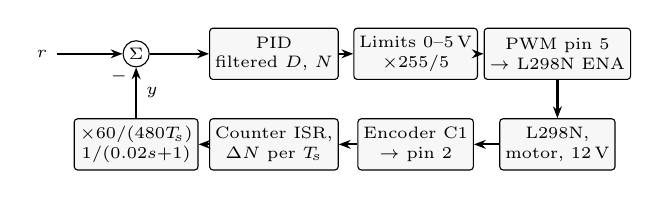
\begin{tikzpicture}[
  box/.style={draw,rounded corners=1.2pt,minimum height=6.5mm,minimum width=1.35cm,font=\fontsize{6}{7}\selectfont,inner sep=2pt,align=center,fill=black!3},
  arr/.style={-{Stealth[length=1.5mm]},thick}]
\node[circle,draw,inner sep=1pt,font=\fontsize{6}{7}\selectfont] (sum) at (0,0) {$\Sigma$};
\node[box] (pid) at (1.75,0) {PID\\ filtered $D$, $N$};
\node[box] (lim) at (3.55,0) {Limits $0$--$5$\,V\\ $\times 255/5$};
\node[box] (pwm) at (5.35,0) {PWM pin 5\\ $\to$ L298N ENA};
\node[box] (mot) at (5.35,-1.15) {L298N,\\ motor, 12\,V};
\node[box] (enc) at (3.55,-1.15) {Encoder C1\\ $\to$ pin 2};
\node[box] (cnt) at (1.75,-1.15) {Counter ISR,\\ $\Delta N$ per $\Ts$};
\node[box] (scl) at (0,-1.15) {$\times60/(480\Ts)$\\ $1/(0.02s{+}1)$};
\draw[arr] (-1.0,0) node[left,font=\fontsize{6}{7}\selectfont]{$r$} -- (sum.west);
\draw[arr] (sum) -- (pid);
\draw[arr] (pid) -- (lim);
\draw[arr] (lim) -- (pwm);
\draw[arr] (pwm) -- (mot);
\draw[arr] (mot) -- (enc);
\draw[arr] (enc) -- (cnt);
\draw[arr] (cnt) -- (scl);
\draw[arr] (scl) -- (sum) node[midway,right,font=\fontsize{6}{7}\selectfont]{$y$};
\node[font=\fontsize{6}{7}\selectfont] at (-0.22,-0.28) {$-$};
\end{tikzpicture}
\caption{Signal chain of the closed loop used in Task~2c: reference $r$ and measured speed $y$ in rpm; controller output in normalised volts.}
\label{fig:chain}
\end{figure}

\emph{Task~1a (open loop).} A constant $255$ feeds the Arduino PWM block on pin 5; the same constant through $5/255$ is logged as the input $u=5$. The encoder interrupt on pin 2 triggers a function-call subsystem that counts edges; a Rate Transition samples the count every $0.02\,\text{s}$; a unit delay and a subtraction give the edges in one sample; the gains $1/0.02$, $1/480$ and $60$ convert to rpm; and the transfer function $1/(0.02s+1)$ follows (the manual's Fig.~1). A two-input scope logs the dataset \code{stepData}.

\emph{Task~1b (closed loop, proportional).} The model has a constant reference, a subtraction, the gain $K$, a saturation $[0,5]$, the gain $255/5$, the PWM block and the same measurement chain. It is the optional hardware check of one chosen $K$ and \emph{was not run}, because no gain meeting the damping targets exists (Section~\ref{sec:t1b}).

\emph{Task~2c (closed loop, PID).} The model of Fig.~\ref{fig:m2c} replaces the gain and saturation by a PID Controller block with the settings of Table~\ref{tab:settings}; the subsystem \emph{Encoder Systems} contains the same measurement chain as Task~1a (confirmed by the group). A scope logs the dataset \code{hw_data} with the reference, the speed and the controller output after saturation.

\begin{figure}[H]
\centering
\figbox{figs/model_task1a.png}{\linewidth}{3.6cm}
\caption{Simulink model of Task~1a (open-loop step and speed measurement chain).}
\label{fig:m1a}
\end{figure}

\begin{figure}[H]
\centering
\figbox{figs/model_task1b.png}{\linewidth}{3.6cm}
\caption{Simulink model of Task~1b (proportional closed loop; not run on hardware).}
\label{fig:m1b}
\end{figure}

\begin{figure}[H]
\centering
\figbox{figs/model_task2c.png}{\linewidth}{3.6cm}
\caption{Simulink model of Task~2c (PID closed loop with the \emph{Encoder Systems} subsystem), after the gain before the PWM block was corrected to $255/5$.}
\label{fig:m2c}
\end{figure}

\subsection{Hardware Wiring}
\begin{table}[H]
\centering
\caption{Wiring used (as reported by the group)}
\label{tab:wiring}
\begin{tabular}{@{}p{2.5cm}p{2.5cm}p{2.8cm}@{}}
\toprule
From & To & Purpose \\
\midrule
Arduino pin 5 & L298N ENA & PWM command \\
L298N IN1 & Arduino 5\,V & Fixed direction \\
L298N IN2 & Arduino GND & Fixed direction \\
L298N outputs & Motor leads & Direct, no series resistor \\
12\,V supply & L298N & Motor power \\
Encoder C1 (yellow) & Arduino pin 2 & Speed pulses (interrupt) \\
Encoder GND (green) & Arduino GND & Return \\
Encoder VCC (blue) & Arduino 5\,V & Encoder supply \\
\bottomrule
\end{tabular}
\end{table}
With IN1 high and IN2 low the bridge drives in one direction only, so the PWM duty on the enable input alone sets the average motor voltage. No circuit diagram was drawn for this experiment; the wiring is given in Table~\ref{tab:wiring} and in the photograph (Fig.~\ref{fig:photo}). The connection of the supply to the driver terminals, the common ground between supply and Arduino, the flyback diode and the motor ratings were not recorded.

\begin{figure}[H]
\centering
\figbox{figs/hw_setup_photo.jpeg}{0.9\linewidth}{4.2cm}
\caption{Photograph of the hardware setup (Arduino Mega 2560, L298N driver, DC encoder motor and $12\,\text{V}$ supply).}
\label{fig:photo}
\end{figure}

\subsection{Analysis Scripts and Saved Files}
Table~\ref{tab:scripts} lists the scripts and Table~\ref{tab:files} the saved logs and results. The scripts share a set of helper functions and write their figures as PNG files into the folder \code{figs}; the code itself is not reproduced here.
\begin{table}[H]
\centering
\caption{Scripts and what they output}
\label{tab:scripts}
\begin{tabular}{@{}p{1.1cm}p{7.0cm}@{}}
\toprule
Task & Script outputs \\
\midrule
1a & Reads \code{stepData}, crops the estimation window to the first $2.5\,\text{s}$ (modified from the full record), runs \code{tfest} with 3 and 2 poles, prints the model, poles with $\omega_n$ and $\zeta$, fit, plateau and DC-gain mismatch; figure: measured against identified step \\
1b & $\Kcr$, $\wcr$ by \code{allmargin} and by Routh; follows the dominant pole as $K$ grows; solves $\zeta=0.707$ and $0.456$; searches critical damping through $dK/ds=0$; \code{stepinfo}; figures: root locus and step responses (line~74 corrected) \\
2a & $\Kcr$ and $\wcr$ by both methods, closed-loop poles at $\Kcr$, sampled critical gain by eigenvalue search; figure: root locus \\
2b & Ziegler--Nichols gains, $L=CG$, closed-loop poles, \code{stepinfo}; sampled and saturated simulation (reference $270\rpm$, $N=50$); figures: root loci, linear and sampled responses \\
2c & Computes the gains for \code{MODE}, sets \code{Kp}, \code{Ki}, \code{Kd}, \code{N}, \code{Ts}, \code{r_ref}; after the run extracts \code{hw_data}, simulates the sampled and the linear loop, computes the specifications, plots and saves (\code{MODE} fixed in the script header) \\
\bottomrule
\end{tabular}
\end{table}

\begin{table}[H]
\centering
\caption{Saved data files (\code{MODE} is P, PI or PID)}
\label{tab:files}
\begin{tabular}{@{}p{3.4cm}p{4.7cm}@{}}
\toprule
File & Content \\
\midrule
\code{Task1a_raw.mat} & Raw $5\,\text{s}$ open-loop log (\code{stepData}) \\
\code{Task1a_Output.mat} & Identified models (3 and 2 poles), plateau, $\Ts$ \\
\code{Task2a_Output.mat} & $\Kcr$, $\wcr$, $\Pcr$, sampled values \\
\code{Task2b_Output.mat} & Gains $K_p,T_i,T_d,K_i,K_d$, $N$, reference \\
\code{Task2c_raw_MODE.mat} & Raw hardware logs (\code{hw_data}) \\
\code{Task2c_MODE.mat} & Processed hardware data ($501$ samples: time, reference, speed, controller output) and specifications \\
\bottomrule
\end{tabular}
\end{table}

% =========================== EXPERIMENTAL PROCEDURE ===========================
\section{Experimental Procedure}

\subsection{Simulation}
\begin{enumerate}
\item Run the Task~1a script on the logged open-loop step to obtain the third-order model and the DC-gain check.
\item Run the Task~1b script on the identified model for the stable range, the damping-ratio gains, critical damping, $\Kcr$ and the root locus.
\item Run the Task~2a script for $\Kcr$, $\wcr$, $\Pcr$ and the sampled critical gain.
\item Run the Task~2b script for the Ziegler--Nichols gains, the root loci of P, PI and PID, the linear step responses and the sampled and saturated simulation.
\end{enumerate}

\subsection{Hardware}
\begin{enumerate}
\item Wire the driver, motor and encoder as in Table~\ref{tab:wiring}; set $\Ts=0.02\,\text{s}$ and the fixed-step solver \code{ode1}.
\item Task~1a: apply a full-duty step to the open-loop model and log the speed. The $10\,\text{s}$ and $15\,\text{s}$ records gave poor fits, so the record was shortened to $5\,\text{s}$ and the script's estimation window to $2.5\,\text{s}$ (Section~\ref{sec:issues}).
\item Task~2c, for each mode in the order P, PI, PID: run the script to compute the gains and set the workspace variables, run the model for $10\,\text{s}$ at $r=270\rpm$, stop it, and run the script again to extract \code{hw_data}, plot and save.
\item Before the closed-loop runs, check that the gain after the controller is $255/5$ and that the controller limits are $0$ and $5$.
\end{enumerate}
The Task~1b hardware check was not executed.

% ========================= OBSERVATION AND DATA RECORDING =========================
\section{Observation and Data Recording}

\subsection{Data Sources and Reading Conventions}
All numbers come from the printed output of the scripts, from the saved \code{.mat} files, or (marked approximate) from the plots. For the hardware runs of Task~2c the quantities are computed over the logged $501$ samples ($10\,\text{s}$ at $0.02\,\text{s}$): the final value is the mean of the last $2\,\text{s}$; the steady-state error is $(r-\text{final})/r$; the overshoot is $(\max-\text{final})/\text{final}$; the \emph{tail peak-to-peak} is the range of the speed over the last $2\,\text{s}$; and the rise time is the script's $10$--$90\%$ value, resolved only to the sample time. One encoder count is $6.25\rpm$. The $\pm2\%$ band around $270\rpm$ is $5.4\rpm$, narrower than one count, so a $2\%$ settling time is not defined for the hardware data (the script returned NaN or the stop time).

\subsection{Task 1a: Open-Loop Step and Identification}
\label{sec:t1a}
A full-duty step ($u=5$) was applied at $t=0$ and the speed was logged for $5\,\text{s}$; the script cropped the estimation window to the first $2.5\,\text{s}$. Table~\ref{tab:idattempts} lists the three identification attempts, and Table~\ref{tab:model} the model that was kept, next to the manual's benchmark. Figure~\ref{fig:id1a} compares the data with the fitted models.

\begin{table}[H]
\centering
\caption{Task 1a identification attempts (measured data, fitted models; script output). The records have $501$, $751$ and $126$ samples.}
\label{tab:idattempts}
\footnotesize
\setlength{\tabcolsep}{3pt}
\begin{tabular}{@{}lcccc@{}}
\toprule
Record & $y_{ss}$ (rpm) & Fit 3p / 2p (\%) & $G(0)$ & Mism. (\%) \\
\midrule
$10\,\text{s}$ & 526.50 & $33.07$ / $-187.41$ & 103.40 & 1.81 \\
$15\,\text{s}$ & 458.25 & $-860.41$ / $18.34$ & 2.19 & 97.61 \\
$5\,\text{s}$, first $2.5\,\text{s}$ (used) & 544.74 & $64.38$ / $61.28$ & 106.31 & 2.42 \\
\bottomrule
\end{tabular}
\end{table}

\begin{table}[H]
\centering
\caption{Identified third-order model of Task 1a (fitted to measured data) against the manual's benchmark identification (study guide values; not our measurement)}
\label{tab:model}
\footnotesize
\begin{tabular}{@{}p{2.3cm}p{3.1cm}p{2.5cm}@{}}
\toprule
Quantity & Ours (M) & Benchmark \\
\midrule
$b_0$ & $7.3108\times10^{6}$ & $5.814\times10^{5}$ \\
$a_2$ & $55.2546$ & $229.5$ \\
$a_1$ & $3570.6$ & $3542$ \\
$a_0$ & $6.877\times10^{4}$ & $1.922\times10^{4}$ \\
Poles (rad/s) & $-24.406$; $-15.424\pm j50.792$ & $-213.3$; $-8.09\pm j4.95$ \\
Pair $\omega_n$, $\zeta$ & $53.08$, $0.291$ (D) & $9.48$, $0.853$ \\
$G(0)$ (rpm/V) & $106.307$ & $30.25$ \\
Fit (\%) & $64.38$ (2 poles: $61.28$) & $79.69$ \\
$\Kcr$ & see Table~\ref{tab:crit} & $1.3651$ \\
$\wcr$ (rad/s) & see Table~\ref{tab:crit} & $59.51$ \\
$\Pcr$ (s) & see Table~\ref{tab:crit} & $0.1056$ \\
\bottomrule
\end{tabular}
\end{table}

\begin{figure}[!htb]
\centering
\figbox{figs/task_1a_identification.png}{\linewidth}{6.6cm}
\caption{Task~1a, measured data and fitted models: measured speed (grey), 3-pole fit (red, $64.4\%$), 2-pole fit (green dashed, $61.3\%$) and plateau (blue dotted) over the first $2.5\,\text{s}$ of a $5\,\text{s}$ full-duty step on the L298N at $12\,\text{V}$ (single run); the lower panel shows the $5\,\text{V}$ input.}
\label{fig:id1a}
\end{figure}

The measured speed reaches about $500\rpm$ within about $0.1\,\text{s}$ and then scatters between about $450$ and $580\rpm$ (approximate, from the plot) with a slow upward drift: the means of consecutive $0.5\,\text{s}$ blocks from $0.5\,\text{s}$ onward are $516.5$, $533.8$, $531.0$ and $560.6\rpm$ (M). Over $1.0$ to $2.5\,\text{s}$ the standard deviation is $25.8\rpm$ and the peak-to-peak range $118.8\rpm$, i.e.\ $19$ counts (M). Both models settle at about $531\rpm\approx5G(0)$, below the plateau mark; the 3-pole model shows a small overshoot near $0.1$ to $0.15\,\text{s}$ that the noisy data do not clearly show.

The stored plateau is $y_{ss}=544.74\rpm$ at $u_{ss}=5\,\text{V}$, so the measured DC gain is $108.948\rpm/\text{V}$ and the model's $G(0)=106.307$ differs by $2.42\%$. Recomputing the mean over $t\ge1.0\,\text{s}$ from the saved window gives $542.0\rpm$ ($0.5\%$ lower), and the last $1.5\,\text{s}$ of the raw $5\,\text{s}$ record average $520.1\rpm$ (D, from the saved files). The block means above lie between $-5.2\%$ and $+2.9\%$ of the stored plateau, so the $2.42\%$ agreement is smaller than the drift of the record, and the plateau is uncertain by a few per cent. The fit of $64.38\%$ is below the benchmark's $79.69\%$, and the 3-pole model improves on the 2-pole model by only $3.1$ percentage points. The script also issued the \code{tfest} warning that the input change should not occur too early relative to the model order, because the step starts at $t=0$ with no pre-step segment.

Figure~\ref{fig:raw15} shows the logged speed of the $15\,\text{s}$ attempt. The speed scatters between about $480$ and $600\rpm$ for about $12.8\,\text{s}$ and then steps down to about $460\rpm$ (approximate); the identification on that record failed (Table~\ref{tab:idattempts}).

\begin{figure}[!htb]
\centering
\figbox{figs/1793467834111_image.png}{\linewidth}{4.7cm}
\caption{Raw logged speed of the $15\,\text{s}$ open-loop attempt (measured, full-duty step, L298N at $12\,\text{V}$, no series resistor): the speed drops at about $12.8\,\text{s}$ (values read from the plot, approximate). This record was not used for identification.}
\label{fig:raw15}
\end{figure}

\subsection{Task 1b: Proportional Design on the Identified Model}
\label{sec:t1b}
Task~1b repeats the items of Pre-Lab Question~2 on the identified model. Table~\ref{tab:t1b} gives what the script printed; Fig.~\ref{fig:rl1b} shows the root locus. The script's step-response figure for the chosen gains is empty (only the reference line), because no gain was found; it is not reproduced.

\begin{table}[H]
\centering
\caption{Task 1b results on the identified model}
\label{tab:t1b}
\footnotesize
\begin{tabular}{@{}p{3.3cm}p{3.7cm}c@{}}
\toprule
Item & Result & Status \\
\midrule
Stable range & $0<K<0.0176$ (\code{allmargin} and Routh) & S \\
Sustained oscillation & $\Kcr=0.0176$, $\wcr=59.755\,\text{rad/s}$, $\Pcr=0.1051\,\text{s}$ & S \\
Gain for $\zeta=0.707$ & Does not exist & S \\
Gain for $20\%$ overshoot & Does not exist ($\zeta=0.456$) & S \\
Critical damping & Does not exist (no real root of $dK/ds=0$ with $0<K<\Kcr$) & S \\
Time-domain specifications & None (no gain to evaluate) & --- \\
Step error, any stable $K$ & $>34.9\%$ & D \\
Hardware check of one $K$ & Not run & N \\
\bottomrule
\end{tabular}
\end{table}

For both damping targets the script states that the open-loop dominant pair, with $\zeta=0.291$, never crosses the target for $0<K<\Kcr$. The step-error bound is $1/(1+\Kcr G(0))=0.349$ from \eqref{eq:essP} with $K\to\Kcr$ (D). The Task~1b script crashed once with an array-size error and was corrected (Section~\ref{sec:issues}); all results above are from the corrected script.

\begin{figure*}[!t]
\centering
\figbox{figs/task_1b_root_locus.png}{0.75\textwidth}{8.3cm}
\caption{Task~1b, root locus of $KG(s)$ for the identified model (simulated): open-loop poles ($\times$), the complex branches running toward the right half-plane, the real branch running left, and the crossing at $\Kcr=0.0176$ (red triangles). Dashed rays are lines of constant $\zeta=0.456$ and $0.707$; the branches never reach them. Left: full view. Right: view from $-40$ to $15$ on the real axis.}
\label{fig:rl1b}
\end{figure*}

\subsection{Task 2a: Critical Gain and Critical Period}
Table~\ref{tab:crit} gives the critical values of the identified model. The two continuous methods agree to four digits. The sampled critical gain, from the discretised loop at $\Ts=0.02\,\text{s}$, is about $75\%$ of the continuous one. The two imaginary-axis poles at $\Kcr$ are at $\pm j59.75\,\text{rad/s}$; the third pole is at $-a_2=-55.25\,\text{rad/s}$ (D), in line with the green square of Fig.~\ref{fig:rl2a}. The sampled critical gain is $0.01318$, which is above the Ziegler--Nichols P gain $0.00879$ by a factor of $1.50$ (D).

\begin{table}[H]
\centering
\caption{Task 2a critical values of the identified model (simulated); sampled at $\Ts=0.02\,\text{s}$}
\label{tab:crit}
\footnotesize
\setlength{\tabcolsep}{3pt}
\begin{tabular}{@{}lcc@{}}
\toprule
Quantity & Continuous & Sampled \\
\midrule
$\Kcr$ (allmargin) & $0.01758$ & $0.01318$ \\
$\Kcr$ (Routh) & $0.01758$ & --- \\
$\wcr$ (rad/s) & $59.7546$ (both methods) & $51.862$ \\
$\Pcr$ (s) & $0.10515$ & --- \\
$\Pcr/\Ts$ & $5.26$ & --- \\
\bottomrule
\end{tabular}
\end{table}

\begin{figure*}[!t]
\centering
\figbox{figs/task_2a_root_locus.png}{0.75\textwidth}{6.4cm}
\caption{Task~2a, root locus of the identified plant with the crossing points $\pm j\wcr$, $\wcr=59.75\,\text{rad/s}$ (red circles) and the closed-loop poles at $\Kcr=0.0176$ (green squares) (simulated). Left: full view. Right: wider view, from $-60$ to $40$ on the real axis, showing the third pole at about $-55$.}
\label{fig:rl2a}
\end{figure*}

\subsection{Task 2b: Ziegler--Nichols Design in Simulation}
Table~\ref{tab:zn} gives the controller parameters from Table~\ref{tab:zn_rules} with $\Kcr=0.01758$ and $\Pcr=0.10515\,\text{s}$; the scripts used the raw Ziegler--Nichols values (the PI scale factors are both $1$) and no detuning was done. Table~\ref{tab:spec} lists the simulated specifications, and Figs.~\ref{fig:rl2b}--\ref{fig:samp2b} the root loci and responses. All three closed loops are stable.

\begin{table}[H]
\centering
\caption{Ziegler--Nichols parameters (derived from $\Kcr$ and $\Pcr$; script values)}
\label{tab:zn}
\footnotesize
\setlength{\tabcolsep}{3.5pt}
\begin{tabular}{@{}lccccc@{}}
\toprule
Mode & $K_p$ & $T_i$ (s) & $T_d$ (s) & $K_i$ & $K_d$ \\
\midrule
P   & $0.008790$ & $\infty$ & $0$ & $0$ & $0$ \\
PI  & $0.007911$ & $0.08763$ & $0$ & $0.09028$ & $0$ \\
PID & $0.01055$ & $0.05258$ & $0.01314$ & $0.2006$ & $1.386\times10^{-4}$ \\
\bottomrule
\end{tabular}
\end{table}

\begin{table}[H]
\centering
\caption{Task 2b simulated specifications (S). Rise time, overshoot (relative to the final value), $2\%$ settling time and error are for the linear continuous model; the peak and tail peak-to-peak are for the sampled simulation with limits at $r=270\rpm$.}
\label{tab:spec}
\footnotesize
\setlength{\tabcolsep}{2.8pt}
\begin{tabular}{@{}lcccccc@{}}
\toprule
Mode & $t_r$ (s) & OS (\%) & $t_s$ (s) & $e_{ss}$ (\%) & Peak (rpm) & Tail p-p (rpm) \\
\midrule
P   & 0.0295 & 39.41 & 0.5925 & 51.69 & 201.2 & 0.0 \\
PI  & 0.1609 & 0.00  & 0.6241 & 0.00  & 271.5 & 0.0 \\
PID & 0.0420 & 5.64  & 0.3408 & 0.00  & 355.7 & 0.2 \\
\bottomrule
\end{tabular}
\end{table}

\begin{figure*}[!t]
\centering
\figbox{figs/task_2b_root_loci.png}{0.85\textwidth}{9.4cm}
\caption{Task~2b, root loci of $L=C(s)G(s)$ for the Ziegler--Nichols P, PI and PID controllers on the identified plant (simulated). Black $\times$: open-loop poles (including the pole at the origin for PI and PID); black $\circ$: controller zeros (at about $-11.4$ for PI and a double zero at about $-38$ for PID); red squares: closed-loop poles at the Ziegler--Nichols gain. All three axes span $-100$ to $20$ on the real axis.}
\label{fig:rl2b}
\end{figure*}

\begin{figure}[!htb]
\centering
\figbox{figs/task_2b_linear_step_responses.png}{\linewidth}{5.3cm}
\caption{Task~2b, linear continuous step responses with the Ziegler--Nichols P, PI and PID controllers on the identified model, normalised by the reference (simulated). P settles at about $0.48$ with ringing, PI approaches $1$ from below, PID overshoots to about $1.06$ (values read from the plot, approximate).}
\label{fig:lin2b}
\end{figure}

\begin{figure}[!htb]
\centering
\figbox{figs/task_2b_discrete_saturated_simulation.png}{\linewidth}{7.3cm}
\caption{Task~2b, sampled and limited simulation ($\Ts=0.02\,\text{s}$, $N=50$, $r=270\rpm$, output limits $0$ and $5$; simulated, no encoder quantization or noise). Top: speed. Bottom: control effort between the limits (dashed). The effort stays inside the limits; the largest value is the initial PID kick of about $4.7\,\text{V}$ (read from the plot).}
\label{fig:samp2b}
\end{figure}

In the sampled simulation the final values are $130.42$, $270.00$ and $270.00\rpm$ for P, PI and PID, and the tail peak-to-peak amplitudes are at most $0.2\rpm$: no sustained oscillation appears.

\subsection{Task 2c: PID Controllers on the Motor}
\label{sec:t2c}
Each controller was run once for $10\,\text{s}$ at $r=270\rpm$ with the gains of Table~\ref{tab:zn}; all runs are after the gain before the PWM block was corrected to $255/5$. Table~\ref{tab:hwlog} lists quantities from the saved logs.

The Task~2c script printed a message that the actuator ``will saturate'' on the initial step (``$K_p r_{\mathrm{ref}}=2.4\,\text{V}\gg5.0\,\text{V}$''); with $K_pr=2.37$, $2.14$ and $2.85\,\text{V}$ these values are below the $5\,\text{V}$ limit, and the logged control samples (Table~\ref{tab:hwlog}) show that the $5\,\text{V}$ limit was never reached in any of the three runs.

\begin{table}[H]
\centering
\caption{Task 2c hardware logs (M): L298N at $12\,\text{V}$, $\Ts=0.02\,\text{s}$, $r=270\rpm$, single run per mode, last $2\,\text{s}$ for the mean, standard deviation and ripple.}
\label{tab:hwlog}
\footnotesize
\setlength{\tabcolsep}{3.5pt}
\begin{tabular}{@{}lccc@{}}
\toprule
Quantity & P & PI & PID \\
\midrule
$K_p$ & $0.00879$ & $0.00791$ & $0.01055$ \\
$K_i$ & $0$ & $0.0903$ & $0.2006$ \\
$K_d$ & $0$ & $0$ & $1.386\times10^{-4}$ \\
First control sample (V) & $2.373$ & $2.136$ & $4.720$ \\
Maximum control (V) & $2.373$ & $2.715$ & $4.720$ \\
Minimum control (V) & $0.450$ & $0.704$ & $0.000$ \\
Mean control (V) & $0.750$ & $1.044$ & $1.017$ \\
Mean speed (rpm) & $184.65$ & $270.17$ & $270.67$ \\
Speed standard deviation (rpm) & $10.5$ & $16.6$ & $25.2$ \\
Speed peak-to-peak (rpm) / counts & $56.3$ / $9$ & $75.0$ / $12$ & $112.5$ / $18$ \\
Control peak-to-peak (V) & $0.494$ & $0.575$ & $1.928$ \\
Samples with control at $0\,\text{V}$ & $0\%$ & $0\%$ & $1.4\%$ \\
Dominant tail frequency (Hz)$^{\ast}$ & $10.9$ & $12.9$ & $13.4$ \\
\bottomrule
\multicolumn{4}{@{}l}{\scriptsize $^{\ast}$Largest FFT peak of the last $2\,\text{s}$; resolution about $0.5\,\text{Hz}$.}
\end{tabular}
\end{table}

\emph{P control} (Fig.~\ref{fig:hwP}). The first control sample is $K_pr=2.373\,\text{V}$. The speed rises to a first peak of $212.5\rpm$ at $0.08\,\text{s}$ (global maximum $218.8\rpm$) and then scatters about a mean of $184.65\rpm$, a steady-state error of $31.61\%$; the simulation settles at $130.42\rpm$ ($51.69\%$) with a steady control of about $1.2\,\text{V}$, whereas the logged mean control is $0.750\,\text{V}$. The rise time is $0.040\,\text{s}$ and the overshoot relative to the final value is $18.5\%$ ($15.1\%$ at the first peak).

\begin{figure}[!htb]
\centering
\figbox{figs/task_2c_p_hardware_vs_simulation.png}{\linewidth}{7.2cm}
\caption{Task~2c, P control on hardware (M) against the sampled and limited simulation and the linear model (S): $K_p=0.00879$, $r=270\rpm$, L298N at $12\,\text{V}$, $\Ts=0.02\,\text{s}$, $N=50$, single run. Top: speed. Bottom: control effort after saturation.}
\label{fig:hwP}
\end{figure}

\emph{PI control} (Fig.~\ref{fig:hwPI}). The first control sample is $2.136\,\text{V}$ and the maximum $2.715\,\text{V}$. The speed has a first peak of $306.3\rpm$ at $0.12\,\text{s}$ ($13.4\%$ above the final value) and a global maximum of $312.5\rpm$ at $1.14\,\text{s}$ ($15.7\%$), and then scatters about $270.17\rpm$ (error $-0.06\%$), with a mean control of $1.044\,\text{V}$ against $2.54\,\text{V}$ ($270/G(0)$, D) in the simulation. The rise time is $0.052\,\text{s}$.

\begin{figure}[!htb]
\centering
\figbox{figs/task_2c_pi_hardware_vs_simulation.png}{\linewidth}{7.2cm}
\caption{Task~2c, PI control on hardware (M) against simulation (S): $K_p=0.00791$, $K_i=0.0903$, $r=270\rpm$, same conditions as Fig.~\ref{fig:hwP}.}
\label{fig:hwPI}
\end{figure}

\emph{PID control} (Fig.~\ref{fig:hwPID}). The first control sample is $4.720\,\text{V}$, equal to $K_pr$ plus the filtered derivative kick $K_dNr$ ($2.848+1.872\,\text{V}$, D), below the $5\,\text{V}$ limit. The speed peaks at $368.8\rpm$ at $0.08\,\text{s}$, $36.6\%$ above the reference ($36.2\%$ above the final value), against $355.7\rpm$ in the sampled simulation, and then oscillates visibly about $270.67\rpm$ (error $-0.25\%$). The control effort swings between $0\,\text{V}$ (reached in $1.4\%$ of the samples) and about $1.9\,\text{V}$ with a mean of $1.017\,\text{V}$. The rise time is $0.0275\,\text{s}$.

\begin{figure}[!htb]
\centering
\figbox{figs/task_2c_pid_hardware_vs_simulation.png}{\linewidth}{7.2cm}
\caption{Task~2c, PID control on hardware (M) against simulation (S): $K_p=0.01055$, $K_i=0.2006$, $K_d=1.386\times10^{-4}$, $N=50$, $r=270\rpm$, same conditions as Fig.~\ref{fig:hwP}.}
\label{fig:hwPID}
\end{figure}

\subsection{Practical Issues Log}
\label{sec:issues}
Only the issues that explain a result or a change of procedure are listed.
\begin{itemize}
\item \textbf{Poor fits and a speed drop in long runs.} The $10\,\text{s}$ record gave a fit of $33.07\%$ and the $15\,\text{s}$ record a failed $3$-pole fit ($-860.41\%$, a pole at about $-2.4\times10^{13}\,\text{rad/s}$); on the $15\,\text{s}$ record the speed dropped mechanically at about $12.8\,\text{s}$ (Fig.~\ref{fig:raw15}). The drop is attributed to the thermal limit of the L298N running without the series resistor; no temperature or current was measured and the run was not repeated. The record was shortened to $5\,\text{s}$ and the estimation window to $2.5\,\text{s}$; the data used are after this change.
\item \textbf{Task~1b script error.} The script stopped with ``Arrays have incompatible sizes'' because the plant has a constant numerator; line~74 was changed to \code{pn = polyder(den)}. Results are after the fix.
\item \textbf{Motor barely turning in Task~2c (P).} The speed stayed at $6.25\rpm$, one encoder count. The cause was the gain before the PWM block set to $5/255$ instead of $255/5$. The reported runs were made after the correction.
\item \textbf{Recycled data in Task~2c (PI).} The first PI output was identical to the P output, because the script cleared the workspace variable \code{MODE}, which fell back to P, and old logs were reused. \code{MODE} was fixed in the script header and the workspace variables were purged; the PI and PID data are after this fix.
\end{itemize}

% ================================ CALCULATIONS ================================
\section{Calculations}

\subsection{Critical Values from the Identified Coefficients}
With $b_0=7.3108\times10^{6}$, $a_2=55.2546$, $a_1=3570.6$ and $a_0=6.877\times10^{4}$, \eqref{eq:kcr} gives (D)
\begin{align}
\Kcr&=\frac{55.2546\cdot3570.6-68770}{7.3108\times10^{6}}=0.01758,\\
\wcr&=\sqrt{3570.6}=59.75\,\text{rad/s},\qquad
\Pcr=\frac{2\pi}{59.75}=0.1051\,\text{s},
\end{align}
equal to the script values. With $G(0)=b_0/a_0=106.31$, the smallest step error of any stable proportional gain is $1/(1+0.01758\cdot106.31)=34.9\%$. For the breakaway condition \eqref{eq:breakaway}, $3s^2+110.51s+3570.6=0$ has the discriminant $110.51^2-12\cdot3570.6=-3.06\times10^{4}<0$, so there is no real breakaway point and critical damping does not exist.

\subsection{Ziegler--Nichols Gains}
From Table~\ref{tab:zn_rules} with $\Kcr=0.01758$ and $\Pcr=0.10515\,\text{s}$ (D):
\begin{align}
\text{P:}\;& K_p=0.5\Kcr=0.008790,\notag\\
\text{PI:}\;& K_p=0.45\Kcr=0.007911,\; T_i=\tfrac{\Pcr}{1.2}=0.08763\,\text{s},\notag\\
& K_i=\tfrac{K_p}{T_i}=0.09028,\notag\\
\text{PID:}\;& K_p=0.6\Kcr=0.01055,\; T_i=0.5\Pcr=0.05258\,\text{s},\notag\\
& T_d=0.125\Pcr=0.01314\,\text{s},\notag\\
& K_i=\tfrac{K_p}{T_i}=0.2006,\; K_d=K_pT_d=1.386\times10^{-4}.
\end{align}
The P loop has $K_pG(0)=0.934$, so \eqref{eq:essP} gives $e_{ss}=1/1.934=51.69\%$ (D), the value found in simulation. The zeros are at $-1/T_i=-11.41$ for PI and $-1/(2T_d)=-38.04$ for PID (D).

\subsection{Closed-Loop Poles at the Ziegler--Nichols Gains}
The scripts printed only stability. The poles of the ideal (unfiltered) loops, recalculated from the identified coefficients while preparing this report (D), are
\begin{itemize}
\item P: $-5.88\pm j54.99$ ($\zeta=0.106$) and $-43.49$;
\item PI: $-5.76\pm j52.92$ ($\zeta=0.108$), $-37.52$ and $-6.21$;
\item PID: $-7.97\pm j58.99$ ($\zeta=0.134$) and $-19.65\pm j5.26$.
\end{itemize}
All lie in the left half-plane, in agreement with the red squares of Fig.~\ref{fig:rl2b}. A recalculation of the linear step responses gives rise times, overshoots and settling times equal to Table~\ref{tab:spec} within $0.1$ percentage point ($39.43\%$ for P and $5.72\%$ for PID, against $39.41\%$ and $5.64\%$).

\subsection{Sampling and Quantization}
The sampled critical gain was recomputed from the zero-order-hold discretisation of the identified model at $\Ts=0.02\,\text{s}$: $0.01318$ at $51.86\,\text{rad/s}$ (D), equal to the script. One encoder count is $60/(480\cdot0.02)=6.25\rpm$, so the tail ranges of $56.25$, $75.0$ and $112.5\rpm$ are $9$, $12$ and $18$ counts. The first PID control sample is $K_pr+K_dNr=0.01055\cdot270+1.386\times10^{-4}\cdot50\cdot270=2.848+1.872=4.720\,\text{V}$.

\subsection{Hardware Readings and Derived Values}
\label{sec:hwcalc}
\emph{Operating-point gain.} The control effort is the normalised voltage that holds the speed, so $y/u$ is the static gain at that operating point (D, from Table~\ref{tab:hwlog}):
\begin{equation}
\tfrac{184.65}{0.750}=246.2,\;
\tfrac{270.17}{1.044}=258.8,\;
\tfrac{270.67}{1.017}=266.1\;\text{rpm/V},
\end{equation}
that is $2.32$, $2.43$ and $2.50$ times $G(0)=106.3\rpm/\text{V}$, whereas the plateau of Task~1a gives $544.74/5=108.9\rpm/\text{V}$. Table~\ref{tab:opp} collects these values. For the P loop, $K_py/u=y/(r-y)=2.164$ is the loop gain at the operating point, against $K_pG(0)=0.934$ in the model.

\emph{Control ripple against speed ripple.} The ratio of the control peak-to-peak to the speed peak-to-peak is $0.494/56.25=0.00878$ (P), $0.575/75.0=0.00767$ (PI) and $1.928/112.5=0.0171$ (PID) (D). The first two equal $K_p$ ($0.00879$, $0.00791$); the PID ratio equals $K_p+K_dN=0.01055+0.00693=0.0175$ within $2\%$.

\emph{Ripple against first-peak excess.} The first peak exceeds the final mean by $27.9$, $36.1$ and $98.1\rpm$ for P, PI and PID, while half the tail peak-to-peak is $28.1$, $37.5$ and $56.3\rpm$ (D).

\emph{Critical gains if only the gain were higher.} If the dynamics of the identified model were unchanged and only the gain were larger by the ratio $2.3$ to $2.5$, the critical gain at the operating point would be $\Kcr/2.5=0.0070$ to $\Kcr/2.3=0.0076$ (continuous) and $0.0053$ to $0.0057$ (sampled) (D). This is a hypothetical scaling, not a measurement.

% ================================== RESULTS ==================================
\section{Results}
Table~\ref{tab:summary} summarises the results by task, Table~\ref{tab:opp} gives the operating-point gains, and Table~\ref{tab:cmp} compares the three controllers in the linear simulation, the sampled simulation and on hardware.

\begin{table}[H]
\centering
\caption{Summary of results by task}
\label{tab:summary}
\footnotesize
\begin{tabular}{@{}p{0.7cm}p{5.3cm}p{1.1cm}@{}}
\toprule
Task & Result & Status \\
\midrule
1a & $G(s)=b_0/(s^3+a_2s^2+a_1s+a_0)$ with the coefficients of Table~\ref{tab:model}; poles $-24.406$, $-15.424\pm j50.792$ & M \\
1a & Fit $64.38\%$ ($61.28\%$ for 2 poles); plateau $544.74\rpm$ at $5\,\text{V}$; DC gain $108.95$ measured, $106.31$ model, mismatch $2.42\%$ & M \\
1b & Stable for $0<K<0.0176$; no gain for $\zeta=0.707$ or $0.456$; no critical damping; step error $>34.9\%$ for any stable $K$; hardware check not run & S, D, N \\
2a & $\Kcr=0.01758$, $\wcr=59.75\,\text{rad/s}$, $\Pcr=0.1051\,\text{s}$; sampled $\Kcr=0.01318$ at $51.86\,\text{rad/s}$ & S \\
2b & Table~\ref{tab:zn}; all three loops stable; PID: rise $0.042\,\text{s}$, $5.64\%$ overshoot, $t_s=0.34\,\text{s}$ & D, S \\
2c & Final speeds $184.65$, $270.17$, $270.67\rpm$ at $r=270\rpm$; errors $31.61\%$, $-0.06\%$, $-0.25\%$ & M \\
\bottomrule
\end{tabular}
\end{table}

\begin{table}[H]
\centering
\caption{Static gain at the operating points (D, from the measured plateau and the logged control effort). $G(0)=106.3\rpm/\text{V}$ for the identified model.}
\label{tab:opp}
\footnotesize
\setlength{\tabcolsep}{3.5pt}
\begin{tabular}{@{}lcccc@{}}
\toprule
Source & $u$ (V) & $y$ (rpm) & $y/u$ (rpm/V) & $y/(uG(0))$ \\
\midrule
Task 1a plateau & 5.000 & 544.74 & 108.9 & 1.02 \\
Task 2c P       & 0.750 & 184.65 & 246.2 & 2.32 \\
Task 2c PI      & 1.044 & 270.17 & 258.8 & 2.43 \\
Task 2c PID     & 1.017 & 270.67 & 266.1 & 2.50 \\
\bottomrule
\end{tabular}
\end{table}

\begin{table*}[!t]
\centering
\caption{Task 2c comparison at $r=270\rpm$: linear continuous simulation (Lin, S), sampled and limited simulation (Smp, S) and hardware (HW, M, single run). OS is the overshoot relative to the final value; ``---'' means not reported by the scripts. Derived entries: Smp overshoot from the printed peak and final value (D).}
\label{tab:cmp}
\scriptsize
\setlength{\tabcolsep}{3pt}
\begin{tabular}{@{}lccccccccc@{}}
\toprule
 & \multicolumn{3}{c}{P} & \multicolumn{3}{c}{PI} & \multicolumn{3}{c}{PID} \\
\cmidrule(lr){2-4}\cmidrule(lr){5-7}\cmidrule(lr){8-10}
Quantity & Lin & Smp & HW & Lin & Smp & HW & Lin & Smp & HW \\
\midrule
Final speed (rpm) & $130.4$ & $130.42$ & $184.65$ & $270.0$ & $270.00$ & $270.17$ & $270.0$ & $270.00$ & $270.67$ \\
$e_{ss}$ (\%) & $51.69$ & $51.69$ & $31.61$ & $0.00$ & $0.00$ & $-0.06$ & $0.00$ & $0.00$ & $-0.25$ \\
Peak speed (rpm) & --- & $201.2$ & $218.8$ & --- & $271.5$ & $312.5$ & --- & $355.7$ & $368.8$ \\
OS (\%) & $39.41$ & $54.3$ & $18.5$ & $0.00$ & $0.6$ & $15.7$ & $5.64$ & $31.7$ & $36.2$ \\
First-peak OS (\%) & --- & --- & $15.1$ & --- & --- & $13.4$ & --- & --- & $36.2$ \\
Rise time (s) & $0.0295$ & --- & $0.040$ & $0.1609$ & --- & $0.052$ & $0.0420$ & --- & $0.0275$ \\
$t_s$, $2\%$ (s) & $0.5925$ & --- & n.d.$^{\ast}$ & $0.6241$ & --- & n.d.$^{\ast}$ & $0.3408$ & --- & n.d.$^{\ast}$ \\
Tail p-p (rpm) & --- & $0.0$ & $56.3$ & --- & $0.0$ & $75.0$ & --- & $0.2$ & $112.5$ \\
Mean control (V) & --- & $\approx1.2$ & $0.750$ & --- & $2.54$ & $1.044$ & --- & $2.54$ & $1.017$ \\
\bottomrule
\end{tabular}\\[3pt]
{\scriptsize $^{\ast}$Not defined: the $\pm2\%$ band ($5.4\rpm$) is narrower than one encoder count ($6.25\rpm$). Lin final speed: $270\cdot0.9344/1.9344$ (D). Sim mean control: $K_p(r-y)$ for P and $r/G(0)$ for PI and PID (D).}
\end{table*}

% ================================= DISCUSSION =================================
\section{Discussion}

\subsection{Steady-State Error and Integral Action}
In simulation the P loop leaves $51.69\%$ error, equal to $1/(1+K_pG(0))$ with $K_pG(0)=0.934$, while PI and PID give zero. On hardware the final speeds are $184.65$, $270.17$ and $270.67\rpm$ (Table~\ref{tab:cmp}): the P error is $31.61\%$, and PI and PID reach the reference within $0.17$ and $0.67\rpm$ ($-0.06\%$ and $-0.25\%$). These offsets are far below one encoder count ($6.25\rpm$) and below the ripple (standard deviation $16.6$ and $25.2\rpm$), so the measurements confirm a zero mean error but not an accuracy better than a few rpm. This agrees with the type argument of Section~\ref{sec:ess}: the integrator removes the error, and a P controller cannot. For the identified model any stable P gain leaves at least $34.9\%$ error, so raising $K_p$ toward $\Kcr$ would not reach zero error and would approach instability.

\subsection{Rise Time, Overshoot and the Derivative Term}
In the linear simulation the rise times are $0.0295$, $0.1609$ and $0.0420\,\text{s}$ for P, PI and PID, the overshoots $39.4\%$, $0\%$ and $5.6\%$, and the $2\%$ settling times $0.59$, $0.62$ and $0.34\,\text{s}$ (Table~\ref{tab:spec}). The PI loop is the slowest to rise because it approaches the reference from below without overshoot; the PID loop is the fastest to settle, which is consistent with the lead from the two PID zeros. The comparison does not isolate the derivative term: the Ziegler--Nichols rules change $K_p$ and $T_i$ between PI and PID as well, and no PID run with $K_d=0$ was made.

On hardware the rise times are $0.040$, $0.052$ and $0.0275\,\text{s}$, resolved to $0.02\,\text{s}$; the P value refers to a lower final speed and is not directly comparable. The PID loop is the fastest. For the overshoot, the first-peak excess over the final mean is $27.9$, $36.1$ and $98.1\rpm$ (Section~\ref{sec:hwcalc}), against half the tail peak-to-peak of $28.1$, $37.5$ and $56.3\rpm$. The P and PI first peaks therefore lie within their own ripple and are not distinguishable from it; only the PID peak ($368.8\rpm$, $36.6\%$ above the reference) is a genuine overshoot, and it agrees with the sampled simulation ($355.7\rpm$, $31.7\%$) to $13\rpm$, two encoder counts. The derivative term thus shortens the rise and settling times in simulation but, together with the higher $K_p$ and the smaller $T_i$, the hardware PID response overshoots most and has the largest ripple. Ziegler--Nichols is a starting point and not a minimum-overshoot design, as the overshoot of the PID loop in simulation and on hardware shows.

\subsection{Theory, Simulation and Hardware}
\emph{Agreement.} (i) $\Kcr$ and $\wcr$ agree between the Routh test, \code{allmargin} and the root locus; the sampled critical gain is $75\%$ of the continuous one, as expected from the $34.2^\circ$ phase lag of the hold at $\wcr$. (ii) The mean error is zero for PI and PID. (iii) The first control samples equal the design values: $K_pr=2.373$ and $2.136\,\text{V}$ for P and PI, and $K_pr+K_dNr=4.720\,\text{V}$ for PID, so the implemented controller matches the design. (iv) The PID first peak agrees with the sampled simulation, as above.

\emph{Disagreement.} (i) The P final speed is $184.65\rpm$ against $130.42\rpm$ in simulation, and the steady controls are $0.750$, $1.044$ and $1.017\,\text{V}$ against about $1.2$, $2.54$ and $2.54\,\text{V}$. The cause is the static gain: $y/u$ is $246$ to $266\rpm/\text{V}$ at the three operating points (Table~\ref{tab:opp}), $2.3$ to $2.5$ times the identified $106.3\rpm/\text{V}$, so the motor needs much less drive at $270\rpm$ than the model predicts. The three values are mutually consistent within $8\%$ (the P point is at $185\rpm$, the other two at $270\rpm$), while the full-duty point gives $109\rpm/\text{V}$; the static curve between the points was not measured, and only three points are available. A plateau depressed by driver heating would reduce this ratio but not remove it, since the first $12\,\text{s}$ of the $15\,\text{s}$ record sit at about the same level (Fig.~\ref{fig:raw15}, approximate). (ii) The ripple of $56$ to $112\rpm$ against at most $0.2\rpm$ (Section~\ref{sec:ripple}). (iii) The PI first-peak overshoot of $13.4\%$ against $0.6\%$ in the sampled simulation, which lies within the ripple. (iv) The $2\%$ settling time, which is undefined on hardware.

The identified model came from a single full-duty step, so its gain is a chord of the static curve between $0$ and $545\rpm$. The Ziegler--Nichols gains designed on it give, at $270\rpm$, loop gains $2.3$ to $2.5$ times larger than designed.

\subsection{Ripple on the Hardware Response}
\label{sec:ripple}
All three runs show a persistent ripple (tail peak-to-peak $56.3$, $75.0$ and $112.5\rpm$, i.e.\ $9$, $12$ and $18$ counts). Four observations bear on its cause.
\begin{enumerate}
\item The open-loop record at full duty scatters by a similar amount (standard deviation $25.8\rpm$, peak-to-peak $118.8\rpm$ over $1.0$ to $2.5\,\text{s}$, including a slow drift), against $25.2$ and $112.5\rpm$ for PID. Measurement noise and quantization alone produce a ripple of this size in the logged speed without any feedback.
\item The logged speed is not smoothed. All logged extrema and ranges are integer multiples of $6.25\rpm$ ($218.75$, $306.25$, $368.75$, $618.75\rpm$; ranges $56.25$, $75.0$, $112.5\rpm$). The manual's Fig.~1 shows a Transfer Fcn $1/(0.02s+1)$ in the speed chain; with the fixed-step solver \code{ode1} at $h=0.02\,\text{s}=\tau$ the Euler update is $y[k+1]=y[k]+(u[k]-y[k])=u[k]$, a one-sample delay with no smoothing (D). This is consistent with the grid, but the block itself was not checked on a model screenshot. If it holds, the encoder steps reach the controller in full.
\item The control ripple is the speed ripple multiplied by the high-frequency controller gain (Section~\ref{sec:hwcalc}): the ratios equal $K_p$ for P and PI and $K_p+K_dN$ for PID, so the derivative term roughly doubles the control ripple. The PID control touches $0\,\text{V}$ in $1.4\%$ of the samples and never reaches $5\,\text{V}$ (maximum $4.720\,\text{V}$).
\item With the loop gain $2.3$ to $2.5$ times higher than designed, the equivalent critical gain would be $0.0070$ to $0.0076$ (continuous) or $0.0053$ to $0.0057$ (sampled), below the three $K_p$ values, which would make the linear loops unstable (hypothetical scaling, Section~\ref{sec:hwcalc}). Against this, the dominant ripple frequencies ($10.9$ to $13.4\,\text{Hz}$, $68$ to $84\,\text{rad/s}$) are above the sampled critical frequency ($8.25\,\text{Hz}$) and similar for the three modes; the estimate comes from one FFT of $2\,\text{s}$ with a $0.5\,\text{Hz}$ resolution and is weak.
\end{enumerate}
The session attributed the ripple to the zero-order hold acting on the $6.25\rpm$ encoder steps together with the actuator limit. The sampled simulation, which contains the hold and the limits, shows no ripple, and the $5\,\text{V}$ limit was not reached, so these two effects do not explain it by themselves; noise passed through the controller gain accounts for its size and for the PID-to-P ratio. A dead zone was also mentioned in the session; no dead-zone width was measured, and the P run holds $184.65\rpm$ at a mean control of $0.750\,\text{V}$, so any dead zone is below that value. The cause of the ripple was not isolated: separating noise from a loop instability would need runs with a smoothed measurement, a lower gain, a longer record and repeats.

\subsection{Root Locus and the Limits of Proportional Control}
The root locus of the identified model explains why Task~1b has no design gain: the dominant pair starts at $\zeta=0.291$ and its damping falls as $K$ rises, so it never reaches $0.456$ or $0.707$, and there is no breakaway point. A proportional gain on this plant therefore trades error against damping in one direction only: the error stays above $34.9\%$ for stable $K$, and the damping decreases as the gain increases. The Ziegler--Nichols P gain gives a gain margin of $2$ in the continuous model but only $1.50$ in the sampled one ($\Kcr^{\mathrm{sampled}}/K_p$, D), and the closed-loop pairs of the P, PI and PID loops are lightly damped ($\zeta=0.11$, $0.11$ and $0.13$, D), which is the source of the $39\%$ overshoot of the P loop in Fig.~\ref{fig:lin2b}. For the manual's reference plant, the study guide's simulation predicts that the PI loop with the same rules is unstable~\cite{studyguide}; for the identified model of this experiment all three loops are stable, which shows how strongly the outcome depends on the identified model.

\subsection{Remarks on the Manual, Models and Scripts}
The following items come from the group's session and from reading the manual~\cite{labmanual}. The verdict of the first two was given in the session; the manual items were not checked with the instructor.
\begin{itemize}
\item \textbf{Task~1b script, line~74 (INCORRECT).} The expression \code{conv(polyder(den), nt) - conv(den, polyder(nt))} fails when the numerator \code{nt} is a scalar, as for a plant without zeros. Corrected to \code{pn = polyder(den)}.
\item \textbf{Task~2c model, gain before the PWM block (INCORRECT).} It was set to $5/255$, which left the motor almost unpowered (speed stuck at $6.25\rpm$). Corrected to $255/5$: the controller output is in normalised volts ($0$ to $5$) and the PWM block expects a duty count ($0$ to $255$).
\item \textbf{Manual, Fig.~2 (NOT CONFIRMED).} The reference identification is shown with \code{iddata(...,0.01)}, a sample time of $0.01\,\text{s}$, while the models and scripts of this experiment use $0.02\,\text{s}$. The sample time given to \code{iddata} must equal that of the logged data, otherwise all time constants of the identified model are scaled by the ratio. The manual's benchmark is therefore not directly comparable with the identified model of this report, unless the manual's model also ran at $0.01\,\text{s}$, which it does not state.
\item \textbf{Manual, Fig.~3 (NOT CONFIRMED).} The caption reads ``Gs=Second Order Transfer Function of DC Motar'' although the figure is the PID block diagram and the task asks for a third-order model; ``Motar'' is a misprint.
\item \textbf{Pre-Lab Question~2 (NOT CONFIRMED).} Its text is not in the manual; Task~1b follows the items as reconstructed in the group's study guide: stable range, gains for $\zeta=0.707$ and for $20\%$ overshoot, critical damping, time-domain specifications and sustained oscillation.
\end{itemize}

\subsection{Sources of Mismatch, Uncertainty and Limitations}
\begin{itemize}
\item \textbf{Single runs.} Each controller was run once at one reference, and the identification step once; no repeat or spread was measured.
\item \textbf{Identification.} The model comes from a $2.5\,\text{s}$ window of one step, with a fit of $64.38\%$, a drifting plateau (block means $516.5$ to $560.6\rpm$) and a step applied at $t=0$. The result depends on the window: the $10\,\text{s}$ record gave $5.3707\times10^{6}/(s^3+43.3866s^2+2800.7s+51944)$, whose critical gain is $0.01295$ and $\wcr=52.92\,\text{rad/s}$ (D), $26\%$ below the used $0.01758$. Every later number inherits this uncertainty. The lightly damped pair ($\zeta=0.29$) may partly describe the sampling delay and not the motor poles; this was not tested.
\item \textbf{Operating point and nonlinearity.} The model is linear and was identified at full duty. The static gain at $185$ to $270\rpm$ is $2.3$ to $2.5$ times larger, and the speed range between $270$ and $545\rpm$ was not measured.
\item \textbf{Resolution and noise.} One encoder count is $6.25\rpm$, larger than the $2\%$ band at $270\rpm$; the speed is not smoothed, and the simulations contain neither quantization nor noise.
\item \textbf{Driver.} The L298N ran without the series resistor and, in the long run, lost speed (attributed to heating); its voltage drop and the supply under load were not measured, and the flyback diode and the PWM frequency were not recorded.
\item \textbf{Tuning.} The Ziegler--Nichols values come from the model's $\Kcr$ and were used without detuning; $\Kcr$ was not found by raising the gain on the real motor.
\item \textbf{Not obtained.} The Task~1b hardware check and any closed-loop run below the Ziegler--Nichols gains.
\end{itemize}

% ================================ CONCLUSION ================================
\section{Conclusion}
A third-order model of the motor, $G(s)=7.3108\times10^{6}/(s^3+55.2546s^2+3570.6s+6.877\times10^{4})$, was fitted to a $2.5\,\text{s}$ window of one $5\,\text{V}$ step (fit $64.38\%$, DC gain within $2.42\%$ of the measured $108.9\rpm/\text{V}$). Its critical values are $\Kcr=0.01758$, $\wcr=59.75\,\text{rad/s}$ and $\Pcr=0.1051\,\text{s}$ (sampled $\Kcr=0.01318$). No proportional gain reaches $\zeta=0.707$ or $0.456$, critical damping does not exist, and any stable P gain leaves at least $34.9\%$ step error. The Ziegler--Nichols P, PI and PID loops are stable in simulation, with errors of $51.69\%$, $0$ and $0$.

On the motor at $270\rpm$, the mean speeds $184.65$, $270.17$ and $270.67\rpm$ show that integral action removes the steady-state error ($31.61\%$ for P, $-0.06\%$ and $-0.25\%$ for PI and PID), and the PID first peak ($368.8\rpm$, $36.6\%$) matches the sampled simulation. The P error is smaller than simulated because the static gain at the operating points is $2.3$ to $2.5$ times the identified gain. A ripple of $56$ to $112\rpm$ peak to peak appears on all hardware responses; it is as large as the open-loop measurement scatter, is multiplied by the controller gain, and its cause was not isolated.

The main limitations are the single operating point and the nonlinear motor behind a linear model, the single runs, the sensitivity of $\Kcr$ to the identification window, and the missing Task~1b hardware check. Improvements would be: identify at the operating speed with a lower step and several records; smooth the speed measurement or use a longer sample time; detune the Ziegler--Nichols gains; measure the critical gain on the hardware; repeat each run; and record the driver temperature or supply current.

% ================================ PRECAUTIONS ================================
\section{Precautions}
\begin{itemize}
\item Before a closed-loop run, check that the gain after the controller is $255/5$ and that the controller limits are $0$ and $5$; the inverse gain leaves the motor almost unpowered.
\item Set \code{MODE} explicitly in the Task~2c script and clear old logs before each run, so that stale data are not analysed.
\item Keep full-duty identification records short ($5\,\text{s}$ here) when the L298N runs without a series resistor, and let the driver cool between runs.
\item Use the same $\Ts$ in the model and in \code{iddata}, and the same measurement chain in the identification and the closed-loop models.
\item Switch the supply on only after the model is ready, keep the shaft clear, keep the encoder wires short and away from the motor leads, and join the grounds of the supply and the Arduino.
\item Identify the plant near the operating speed that will be used in the closed-loop tests.
\end{itemize}

% ================================ REFERENCES ================================
\begin{thebibliography}{99}

\bibitem{labmanual}
Dr. Y. V. Karteek, ``Experiment 9: Steady State Error using Root Locus Design,'' \textit{EE302 Control Systems Laboratory Manual}, Indian Institute of Technology Mandi, Aug.--Dec. 2026.

\bibitem{studyguide}
``EE302 Lab 9: Steady-State Error using Root Locus Design, study guide for the lab and the viva,'' group document, Indian Institute of Technology Mandi, Aug.--Dec. 2026.

\bibitem{ogata}
K. Ogata, \textit{Modern Control Engineering}, 5th ed. Upper Saddle River, NJ, USA: Prentice Hall, 2010.

\bibitem{franklin}
G. F. Franklin, J. D. Powell, and A. Emami-Naeini, \textit{Feedback Control of Dynamic Systems}, 8th ed. New York, NY, USA: Pearson, 2019.

\bibitem{zn}
J. G. Ziegler and N. B. Nichols, ``Optimum settings for automatic controllers,'' \textit{Trans. ASME}, vol. 64, pp. 759--768, 1942.

\bibitem{arduino_mega}
Arduino, ``Arduino Mega 2560 Rev3,'' [Online]. Available: \url{https://docs.arduino.cc/hardware/mega-2560}

\bibitem{mw_arduino}
MathWorks, ``Simulink Support Package for Arduino Hardware,'' [Online]. Available: \url{https://www.mathworks.com/hardware-support/arduino-simulink.html}

\bibitem{mw_sysid}
MathWorks, ``System Identification Toolbox,'' Documentation, [Online]. Available: \url{https://www.mathworks.com/products/sysid.html}

\bibitem{l298}
STMicroelectronics, ``L298 Dual Full-Bridge Driver,'' datasheet.

\end{thebibliography}

\end{document}
